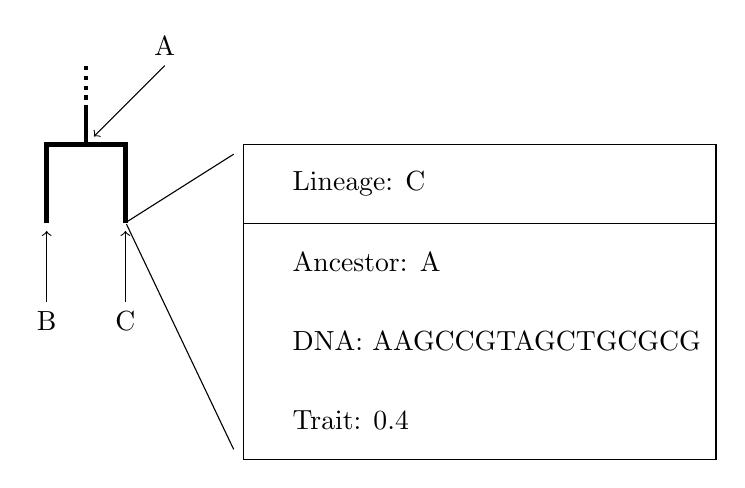
\begin{tikzpicture} 
  % Phylogeny
  \draw[ultra thick,dotted] (0,1) node {}  -- (0, 0.5) node {}; 
  \draw[ultra thick] (0,0.5) node {}  -- (0, 0) node {}; 
  \draw[ultra thick] (-0.5,-1) node {} -- (-0.5, 0) node {} -- (0.5, 0) node {} -- (0.5, -1) node {}; 
  % Arrows
  \draw[->] (1,1) node[anchor=south] {A} -- (0+0.1,0+0.1) node {};
  \draw[->] (-0.5,-2) node[anchor=north] {B} -- (-0.5,-1-0.1) node {};
  \draw[->] ( 0.5,-2) node[anchor=north] {C} -- ( 0.5,-1-0.1) node {};
  % Zoomer
  % Zoom on endpoint of phylogeny
  \draw[] ( 0.5+0.0125,-1+0.0125) node {} -- (2.0-0.125, 0.0-0.125) node {};
  \draw[] ( 0.5+0.0125,-1-0.0125) node {} -- (2.0-0.125,-4.0+0.125) node {};
  % Zoom on C
  % \draw[] ( 0.5+0.125,-2.25+0.25) node {} -- (2.0-0.125, 0.0-0.125) node {};
  % \draw[] ( 0.5+0.125,-2.25-0.25) node {} -- (2.0-0.125,-4.0+0.125) node {};
  % Rectangle
  \draw[] (2.0,-4.0) rectangle (8.0,0.0); 
  \draw[] (2.0,-1.0) rectangle (8.0,0.0); 
  \node[anchor=west] at (2.5,-0.5) {Lineage: C};
  \node[anchor=west] at (2.5,-1.5) {Ancestor: A};
  \node[anchor=west] at (2.5,-2.5) {DNA: AAGCCGTAGCTGCGCG};
  \node[anchor=west] at (2.5,-3.5) {Trait: 0.4};
\end{tikzpicture}